\chapter{总体设计}
\section{软件描述}
我们的云音乐系统包括前台和后台两个部分。

前台主要功能是:
向用户显示必要的图形信息,对用户的输入进行处理,向
后台进行请求。
这些请求包括:
对于播放状态的调整(单用户行为)、
对于软件界面的控制(单用户行为)、
发布对于歌曲的附加信息的改变,如评分、评价(网络行为)、
管理本地的数据内容,如歌曲、歌单(单用户行为)、
对歌曲请求下载(网络行为)
等。
并且对于音乐的播放界面,需要根据模仿进度、播放的曲目
进行播放界面的调整,需要改变进度条、曲目封面等界面元素。
对于支付系统,前台需要完成用户登录、订单确认、订单信息显示
等功能,这一部分同样需要前后台的互相交互。

后台主要功能是:
响应前台的请求,对于前台的操作做出的对于本地数据的改变,
根据一定的策略进行同步(无论是单用户行为还是网络行为)。
对于网络行为,后台需要同时完成用户登录凭据相关的确认,
并且在凭据失效时,向前台发送重登录的提示。

本章节中,我们将详细显示这些具体的设计要求。

\newpage
\section{处理流程}
\subsection{总体流程}

\begin{figure}[h]
\centering
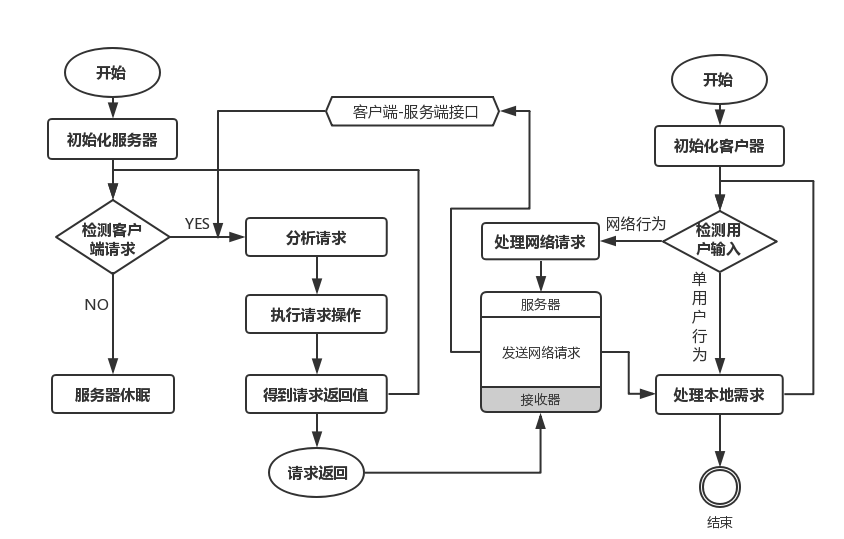
\includegraphics[width=15cm]{images/do_1}
\caption{总体流程图}
\end{figure}

我们的软件需要服务器端与客户端的交互作用,
可以从此图中看到,服务器需要保持长时间的高响应状态,
并且,从客户端输入的请求时不定时、无规律的,
所以我们的服务端在响应请求时,需要动态的根据一定时间段内的
请求数量以及请求类型进行相应的服务调整,
比如,调整自动选择的音质、画质的输出,
自动调整非紧急的下载任务,或调低相应响应速度。

需要注意的是,为了客户端的服务模型的一致性与可重用性,
网络行为与单用户行为(本地行为)有一定的重叠,
这种服务模型可以提高我们的软件行为一致性。

\newpage
\subsection{系统基本流程}
\begin{figure}[h!]
\centering
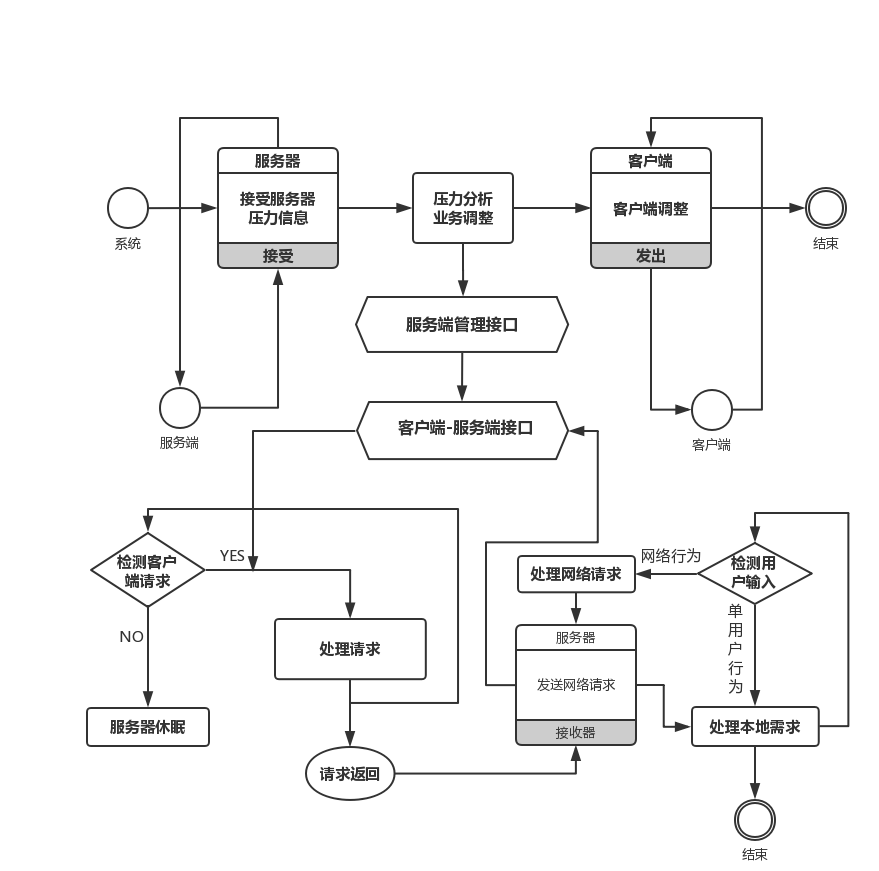
\includegraphics[width=15cm]{images/do_2}
\caption{系统基本流程图}
\end{figure}

我们的系统作为服务短语客户端之间的管理系统,
会动态的根据服务器的状态,
 当前的请求压力,对于服务端以及客户端的行为做出调整。

 如图所示,服务端和客服端对于系统同时有数据输入与输出,
 而我们的系统,根据这些信息会做出决断。

\newpage
\subsection{客户端基本流程}
\begin{figure}[h!]
\centering
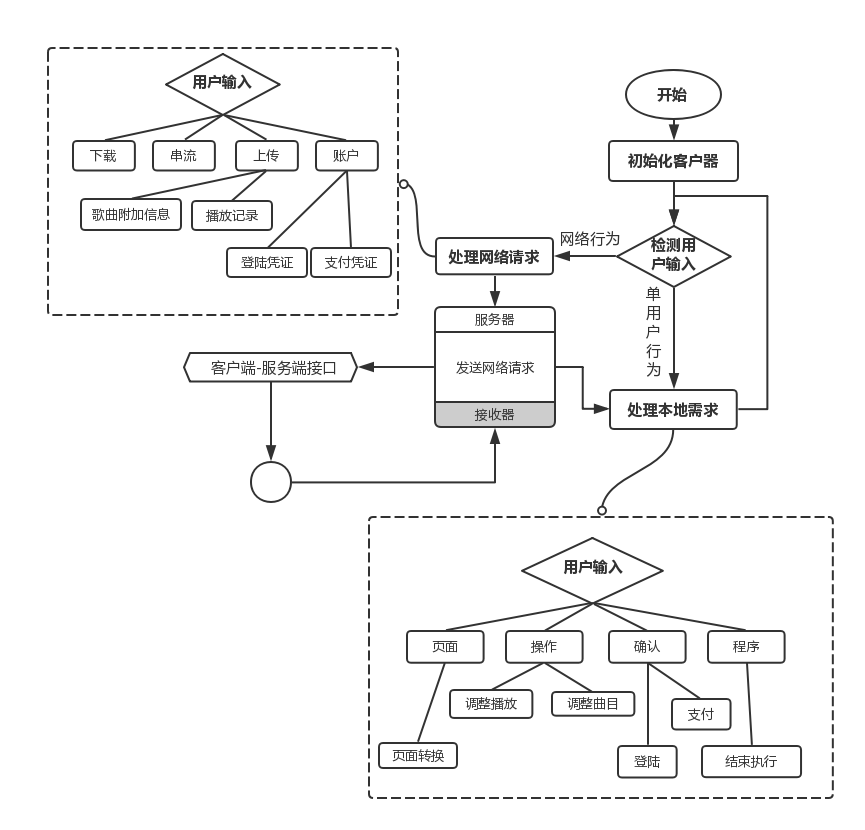
\includegraphics[width=15cm]{images/do_3}
\caption{客户端基本流程图}
\end{figure}

本图中,我们列出了客户端的基本处理流程。

可以看到,在客户端的服务流程模式中,我们需要对于网络请求,
可能有下载或串流的\textbf{大文件低频率型}请求,
也有上传用户对歌曲做出的评分、评价等
\textbf{小文件高频率型}数据需求。
对于这些不同的数据特征,需要有与服务器交互时的不同策略。

对于单用户本地输入,我们的实现方式可以较为随意,
因为满足要求即可,而不会牵扯到服务端以及系统级别的服务
的改变。

\newpage
\subsection{服务器端基本流程}
\begin{figure}[h!]
\centering
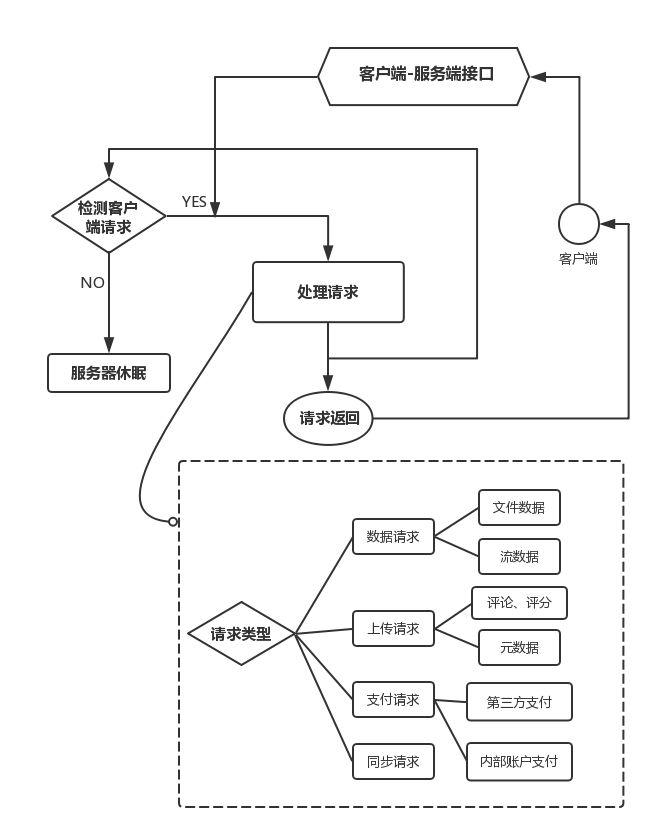
\includegraphics[width=13cm]{images/do_4}
\caption{服务端基本流程图}
\end{figure}

本图中,我们列出了服务器端的基本处理流程。

对于服务器的任务,我们可以将其大致分为四个部分,
分别对应着四种请求,即:数据请求、上传请求、
支付请求、同步请求。对于这四种请求,我们将使用不同的模块
来分别对其进行响应。

\newpage
\subsection{客户端功能具体流程}
\subsubsection{页面转换} % (fold)
\label{ssub:页面转换}
用户通过用户图形界面中的控制元素,
如,对于PC端,使用鼠标点击页面的转换按钮,
或对于移动客户端,触摸相应的按钮或大幅度两侧滑动界面,
需要使得客户端响应这样的输入,
做到相应的页面转换,
由于音乐客户端的特殊性,
我们需要满足在各个页面下够可以播放房钱正在收听的音乐,
所以,无论是网页客户端还是移动客户端,
我们都需要增加迷你播放器,
来在不是歌曲播放界面的页面中给予用户方便地控制、切换、调整播放行为的方式。
% subsubsection 页面转换 (end)

\subsubsection{歌曲操作} % (fold)
\label{ssub:歌曲操作}
歌曲操作对应于两种情形:

首先,在真实的完整播放界面中,我们需要给予用户完整的播放控制能力,
包括:
\begin{enumerate}
    \item 精确控制进度条:(在移动端)控制条的拖动速度可以通过
    触摸位置与进度条的相对垂直距离来控制,具体要求见第七章;
    \item 切换播放/暂停状态;
    \item 切换歌曲列表的播放模式:包括顺序播放、随机播放、列表循环。
    \item 下一曲/上一曲;
\end{enumerate}

而对于其他页面下的迷你播放器,功能上可以有所放松,
比如,精确控制进度条的功能可以不实现。
% subsubsection 歌曲操作 (end)

\subsubsection{登陆操作} % (fold)
\label{ssub:登陆操作}
用户在用户登录界面输入账号和密码,客户端前端需要将登录信息做严格加密后,由后端接口
向服务器端传递登录信息,并获取服务器的返回结果。
根据返回结果,需要做以下处理:
\begin{enumerate}
    \item \textbf{登录成功}:显示正确的提示信息,并对账户界面做相应的调整。
    \item \textbf{因凭据错误登陆失败}:告知用户错误的原因,并提示重试或修改密码。
    \item \textbf{因用户不存在而登录失败}:告知用户用户名不存在,并提示是否要注册账户。
    \item \textbf{服务器响应错误}:告知用户相应的信息,并提示用户检查网络状态并重试。
\end{enumerate}
% subsubsection 登陆操作 (end)

\subsubsection{支付操作} % (fold)
\label{ssub:支付操作}
对于前端完成的订单信息,客户端应该对齐进行初步验证完整性、正确性后,
进行加密并通过后端接口向服务器进行验证。
根据返回结果,可能需要做以下处理:
\begin{enumerate}
    \item \textbf{支付成功}:显示正确的提示信息,
        并对账户界面和可用歌曲的内容做相应的调整。
    \item \textbf{因账户余额不足错导致支付失败}:告知用户错误的原因,
        并提示重试或充值。
    \item \textbf{因第三方支付验证失败错导致支付失败}:告知用户错误的原因,
        并提示重试或改变支付方式。
    \item \textbf{服务器响应错误}:告知用户相应的信息,并提示用户检查网络状态并重试。
\end{enumerate}
% subsubsection 支付操作 (end)

\subsubsection{程序控制操作} % (fold)
\label{ssub:程序控制操作}
对于程序本身的控制,我们需要完成对程序的关闭、重启、更新等操作,
这些操作涉及到不同的平台的不同操作模式。而对于Web网页客户端,
往往没有这些需求,但是,由于关闭或者刷新网页产生的类似
关闭、重启的操作,也需要进行用户行为数据的记录。
% subsubsection 程序控制操作 (end)

\subsection{服务器端功能具体流程}
\subsubsection{数据请求} % (fold)
\label{ssub:数据请求}
对于客户端传递的数据请求,可以分为
文件数据和流数据两种情形:

对于文件数据,使用的技术较为传统,只需要与客户端建立稳定的HTTP/HTTPS连接,
并传递相应的文件。因为音乐文件的大小一般不会过大,所以我们一般不需要在
客户端对于单个客户端的文件数据请求建立多信道或者多线程的连接,
但是在客户端,需要对不同文件的接收做出相应的多线程支持,
但同时下载的文件个数须有一定限制,为了减少服务器压力并充分利用客户端的网络资源。

对于流数据,我们需要考虑到数据传输通道的随时可能关闭以及随时可能需要改编数据抽取位置,
所以应当对于其灵活性作出充分设计。
% subsubsection 数据请求 (end)

\subsubsection{上传请求} % (fold)
\label{ssub:上传请求}
用户在使用软件的过程中,会高频率产生上传的信息,对于评论、评分这些对应到歌曲的
信息,需要实时的对全体网络的用户产生影响,
所以我们应该建立与数据库的专用接口,并且,通过短时间内对于同一首歌的评论、评分
进行缓存、预处理,来减少对于数据库的高频访问。

而对于,用户的浏览记录、播放记录、偏好设置等等,由于没有实施改变的需求,
我们可以利用同步机制,在程序关闭、用户登出、定时器触发计时的情形下
对其进行同步,从而减少服务器压力。
% subsubsection 上传请求 (end)

\subsubsection{支付请求} % (fold)
\label{ssub:支付请求}
客户端提出的支付请求,有可能被主动篡改或者对第三方攻击者恶意篡改,
所以我们需要对其进行严格的验证。

对于账户内部支付(余额支付),我们需要验证用户的登陆凭据,以及
账户数据库内的余额信息是否足够支付订单。对于可疑的订单行为
(如高频购买、重复购买、数额巨大订单这样的客户端理应不可能
发出的订单信息)
我们应对其进行黑名单阻挡。

对于第三方支付的账单,我们需要通过第三方支付平台的相应接口来
对其进行正确性、完整性的审查,并做出正确的反馈。
% subsubsection 支付请求 (end)

\newpage
\section{功能结构设计}
\subsection{整体结构}

我们的系统分为以下模块:

\begin{figure}[h!]
\centering
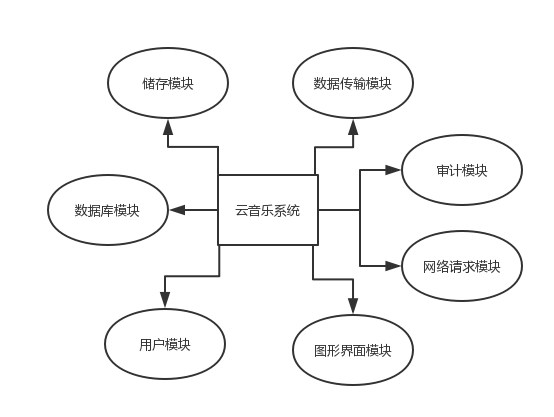
\includegraphics[width=13cm]{images/do_5}
\caption{系统模块结构图}
\end{figure}

\begin{table}[h]
\centering
\caption{系统模块结构表} 
\begin{tabular}{|c|c|}
    \hline
    模块ID & 模块名称 \\
    \hline
    M.CLOUDMUSIC.001 & 储存模块 \\
    M.CLOUDMUSIC.002 & 数据库模块 \\
    M.CLOUDMUSIC.003 & 用户模块 \\
    M.CLOUDMUSIC.004 & 图形界面模块 \\
    M.CLOUDMUSIC.005 & 数据传输模块 \\
    M.CLOUDMUSIC.006 & 审计模块 \\
    M.CLOUDMUSIC.007 & 网络请求模块 \\
    \hline
\end{tabular}
\end{table}

如图和表所示,我们分别简单描述这些模块的作用和范围:

\subsection{M.CLOUDMUSIC.001 储存模块}
\begin{itemize}
    \item 储存歌曲文件;
    \item 储存歌曲元信息,如评论、评分、下载数据、支付数据;
    \item 存储网络缓存;
    \item 存储数据库文件本身。
\end{itemize}

\subsection{M.CLOUDMUSIC.002 数据库模块}
\begin{itemize}
    \item 根据用户的请求,生成不同的数据库查询语句;
    \item 检测用户权限是否满足,若满足则发送给数据库并接收结果,否则报告错误
        并向审计模块报告越权行为;
    \item 对数据库进行高频率的更新,需要对特定用途的查询或更新设计专用的
        存储过程或触发器;
    \item 定时审计,需要与审计模块密切联系。
\end{itemize}

\subsection{M.CLOUDMUSIC.003 用户模块}
\begin{itemize}
    \item 存储用户的信息;
    \item 响应高频度的用户登录凭证验证查询任务;
    \item 动态更新用户信息的变化;
    \item 对于新用户注册,要及时进行数据更新,保证可用性。
\end{itemize}

\subsection{M.CLOUDMUSIC.004 图形界面模块}
\begin{itemize}
    \item 处理用户与图形界面的交互;
    \item 处理前端所执行的结果向服务端的发送;
    \item 处理后端接收到的服务器命令对于界面的实时变化;
    \item 对于较复杂的界面交互、动画,需要平衡性能与效果。
\end{itemize}

\subsection{M.CLOUDMUSIC.005 数据传输模块}
\begin{itemize}
    \item 对于高频小文件(HFLS, High Frequency Low Size)
        传输,保证高可用、低延迟;
    \item 对于低频大文件(LFHS, Low Frequency High Size)
        传输,保证高带宽、低重传;
\end{itemize}

\subsection{M.CLOUDMUSIC.006 审计模块}
\begin{itemize}
    \item 审计数据库模块的越权查询行为;
    \item 审计支付过程中的可疑订单、可疑账户;
    \item 审计网络请求模块中的受篡改请求、恶意请求(如
        分布式拒绝服务(DDoS:Distributed Denial of Service))。
\end{itemize}

\subsection{M.CLOUDMUSIC.007 网络请求模块}
\begin{itemize}
    \item 处理服务器与客户端之间的请求交互;
    \item 处理分布式储存系统之间的同步、传输请求;
    \item 处理本地ISP与顶级ISP之间的网络服务调配。
\end{itemize}

\newpage

\section{功能需求与程序代码的关系}
\begin{table}[htbp]
\centering
\caption{功能需求与程序代码的关系表} \label{tab:requirement-module}
\small

\begin{tabular}{|c|c|c|c|c|c|c|c|}

    \hline
    功能 &              储存 & 数据库 & 用户 & 图形界面 & 数据传输 & 审计 & 网络请求 \\
    \hline
    SYS.001 客户端启动 &   Y &    •   & •    &     Y    &    •     &  •   &   •      \\
    \hline
    SYS.002 客户端关闭 &   Y &    •   & •    &     Y    &    •     &  •   &   •      \\
    \hline
    SYS.003 客户端升级 &   Y &    •   & •    &     Y    &    Y     &  •   &   Y      \\
    \hline
    USER.001 用户登录  &   Y &    Y   & Y    &     Y    &    •     &  Y   &   Y      \\
    \hline
    USER.002 用户注册  &   Y &    Y   & Y    &     Y    &    •     &  Y   &   Y      \\
    \hline
    USER.003 用户注销  &   Y &    Y   & Y    &     Y    &    •     &  Y   &   Y      \\
    \hline
APP.001 生成主页界面   &   • &    •   & •    &     Y    &    •     &  •   &   •      \\
    \hline
APP.002 生成音乐集界面 &   • &    •   & •    &     Y    &    •     &  •   &   •      \\
    \hline
APP.003 生成音乐播放界面 & • &    •   & •    &     Y    &    •     &  •   &   •      \\
    \hline
APP.004 生成音乐推荐界面 & • &    Y   & Y    &     Y    &    Y     &  •   &   Y      \\
    \hline
APP.005 生成账户界面   &   • &    Y   & Y    &     Y    &    Y     &  •   &   Y      \\
    \hline
APP.006 生成设置界面   &   • &    •   & •    &     Y    &    •     &  •   &   •      \\
    \hline
MUSIC.001 音乐播放控制 &   Y &    Y   & •    &     Y    &    Y     &  •   &   Y      \\
    \hline
MUSIC.002 音乐串流控制 &   Y &    Y   & •    &     Y    &    Y     &  •   &   Y      \\
    \hline
MUSIC.003 音乐下载控制 &   Y &    Y   & •    &     Y    &    Y     &  •   &   Y      \\
    \hline
    SHOP.001 购买音乐  &   • &    Y   & Y    &     Y    &    •     &  Y   &   Y      \\
    \hline
    SHOP.002 购买订阅  &   • &    Y   & Y    &     Y    &    •     &  Y   &   Y      \\
    \hline
SYNC.001 数据同步上传  &   Y &    •   & Y    &     •    &    •     &  Y   &   Y      \\
    \hline
SYNC.002 数据同步下载  &   Y &    •   & Y    &     •    &    •     &  Y   &   Y      \\
    \hline

\end{tabular}
\note{各项功能需求的实现与各个程序模块的分配关系}
\end{table}